% Chapter 1

\chapter{Theoretical aspects}

\label{ch:classicpercolation} % For referencing the chapter elsewhere, use \autoref{ch:introduction}

%----------------------------------------------------------------------------------------

%----------------------------------------------------------------------------------------

\section{Setup}

A lattice $(G, N, S)$ is set of nodes $G$, a neighbour relation $N$ from $G$ to to the power set of $G$: $N \colon G \to \mathcal{P}(G)$, and a state map $S \colon G \to Q \subseteq \mathbb{N}$. The precise nature of $G$ and $N$ depends on exactly what type of lattice we're considering. For simplicity, our analysis and results here will be limited to a 2D square lattice, which can be either infinite or finite.
In this case, $G$ is a subset of the set of ordered pairs of natural numbers: 
\begin{equation}
    G \subseteq \mathbb{N} \times \mathbb{N} = \{(i, j) \mid i, j \in \mathbb{N}\}
\end{equation}

So, for example, $(3, 2)$ and $(8843, 0)$ could be elements of $G$.
If we're considering an infinite lattice, then we have 

$$ 
G = \mathbb{N} \times \mathbb{N}
$$ 

$N$ specifies a set of neighbours for each element of $G$. If one views the lattice as a graph, then $N$ contains information about the edges of the graph. In the (infinite) 2D square lattice case, we have 
\begin{equation}
\begin{gathered}
N \colon G \to \mathcal{P}(G) \\
(i, j) \mapsto \{ (i-1, j), (i+1, j), (i, j-1), (i, j+1) \} 
\end{gathered}
\end{equation}

For every node in $G$, this map assigns 4 neighbours. If one thinks of the lattice as a grid, then for every node $(i, j)$ this map assigns the left, right, top and bottom nodes as its neighbours.

$S$ simply assigns a "state" in the set $Q$ to each node in $G$. In standard percolation theory, each node can be in one of two states, so $Q = \{0, 1\}$. These two states are also called dead/alive, black/white or active/inactive.

A cluster $C$ in the lattice is defined as a subset of connected nodes $(i, j)$ in the lattice with such that $S(i, j) = 1$. Connected here means that for every pair $(i_1, j_1) \in C$ and $(i_2, j_2) \in C$ there exists a sequence of neighbouring nodes with $(i_1, j_1)$ being the first item in the sequence and $(i_2, j_2)$ being the last.



\section{Percolation}

\begin{figure}[h]
  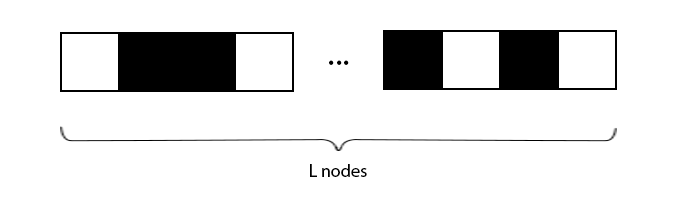
\includegraphics[width=\linewidth]{Images/1dlattice.png}
  \caption{A 1D lattice of size L, with a few dead nodes}
  \label{fig:1dlattice}
\end{figure}




Percolation theory refers to the study of the structure of clusters formed in the lattice, given some choice of state map $S$. In standard percolation theory, one randomly (with probability $p$) assigns either state $0$ or state $1$ to each and every node in the lattice. Under these circumstances, the system presents a phase transition, when one varies the occupation probability $p$. There exists a critical value $p_c$ such that for $p > p_c$, the infinite lattice is said to "percolate", i.e. clusters spanning the whole lattice appear. For the 2D square lattice, the threshold is $p_c = 0.59274621(13)$. This number changes for different choices of $G$ and $N$.


\autoref{fig:1dlattice} and \autoref{fig:2dlattice} provide examples of percolation in 1D and 2D lattices.





In biology, percolation theory has been used to successfully predict the fragmentation of biological virus shells (REF), with the percolation threshold of Hepatitis B virus capsid predicted and detected experimentally (REF). In environmental science, percolation theory has been applied to studies of how environment fragmentation impacts animal habitats (REF) and models of how the plague bacterium Yersinia pestis spreads (REF).


Our goal will be to study the behavior of some quantities of interest associated with percolation models.

\begin{figure}[H]
  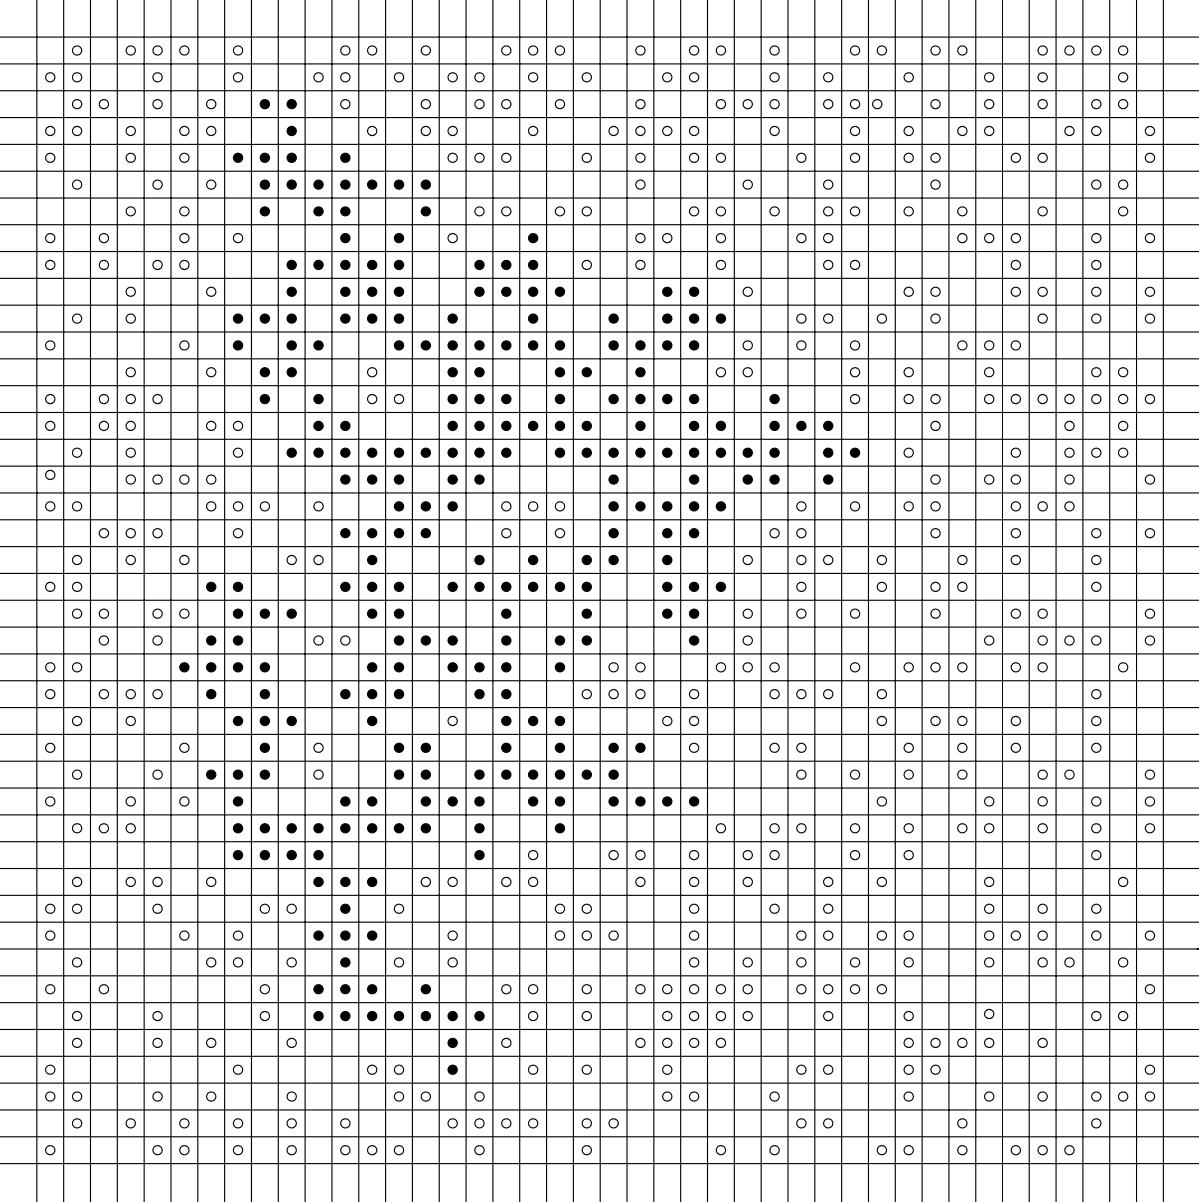
\includegraphics[width=\linewidth]{Images/2dlattice.png}
  \caption{A finite piece of an infinite 2D lattice. The largest cluster is made up of the nodes with circles painted, while the smaller clusters are denoted by open circles.}
  \label{fig:2dlattice}
\end{figure}

\section{Percolating cluster strength}
\label{sec:th_percolating_cluster_strength}

The first interesting quantity we can look at is the percolating strength $P(p)$. This quantity  represents the probability that a randomly picked node belongs to the percolating cluster. Another way to think of this quantity is that it represents the fraction of the whole lattice that is covered by the percolating cluster. 

For small values of $p$, all islands are finite. Starting at any randomly site, it is impossible to get arbitrarily far away by walking only along the connected sites. As we increase $p$, the largest cluster becomes infinite at a precise value $p = p_c$. When this happens, it is possible to get arbitrarily far from a starting point in the infinite cluster by walking along the connected sites. For $p < p_c$, there are no infinite clusters, so $P(p)$ vanishes. However, for $p > p_c$, $P(p)$ monotonically increases. For $1 \gg (p - p_c) > 0$, that is, for $p$ greater  but close to $p_c$, we have (REF 1):

$$
    P(p) \propto (p - p_c)^\beta 
$$

The qualitative behaviour of $P(p)$ can be seen in figure (FIG 1)


$\beta$ is a universal critical exponent which depends only on the lattice dimension, and not on its geometry. In 2 dimensions, $\beta = \frac{5}{36}$, is the same for the square, hexagonal, or any other geometry (REF 1). 

P(p) is one of the order parameters for percolating systems, since it is zero for $p < p_c$, and non-zero for $p > p_c$.


\section{Mean cluster size}
\label{sec:th_mean_cluster_size}

Another interesting quantity is $\chi(p)$, the mean cluster size, which is the average number of nodes in among finite clusters. One can think of each node in the cluster as having one "unit of mass", in which case the mean cluster size represents the average mass. Just like $P(p)$, for $\chi(p)$, we have

$$ 
    \chi(p) \propto  |p - p_c|^{-\gamma} \textrm{,} \hspace{0.35cm}  \textrm{for} \hspace{0.15cm} |p - p_c| \ll 1 
$$ 

The qualitative behaviour of $\chi(p)$ can be seen in \autoref{fig:mean_cluster_size_1}
.

\begin{figure}[H]
  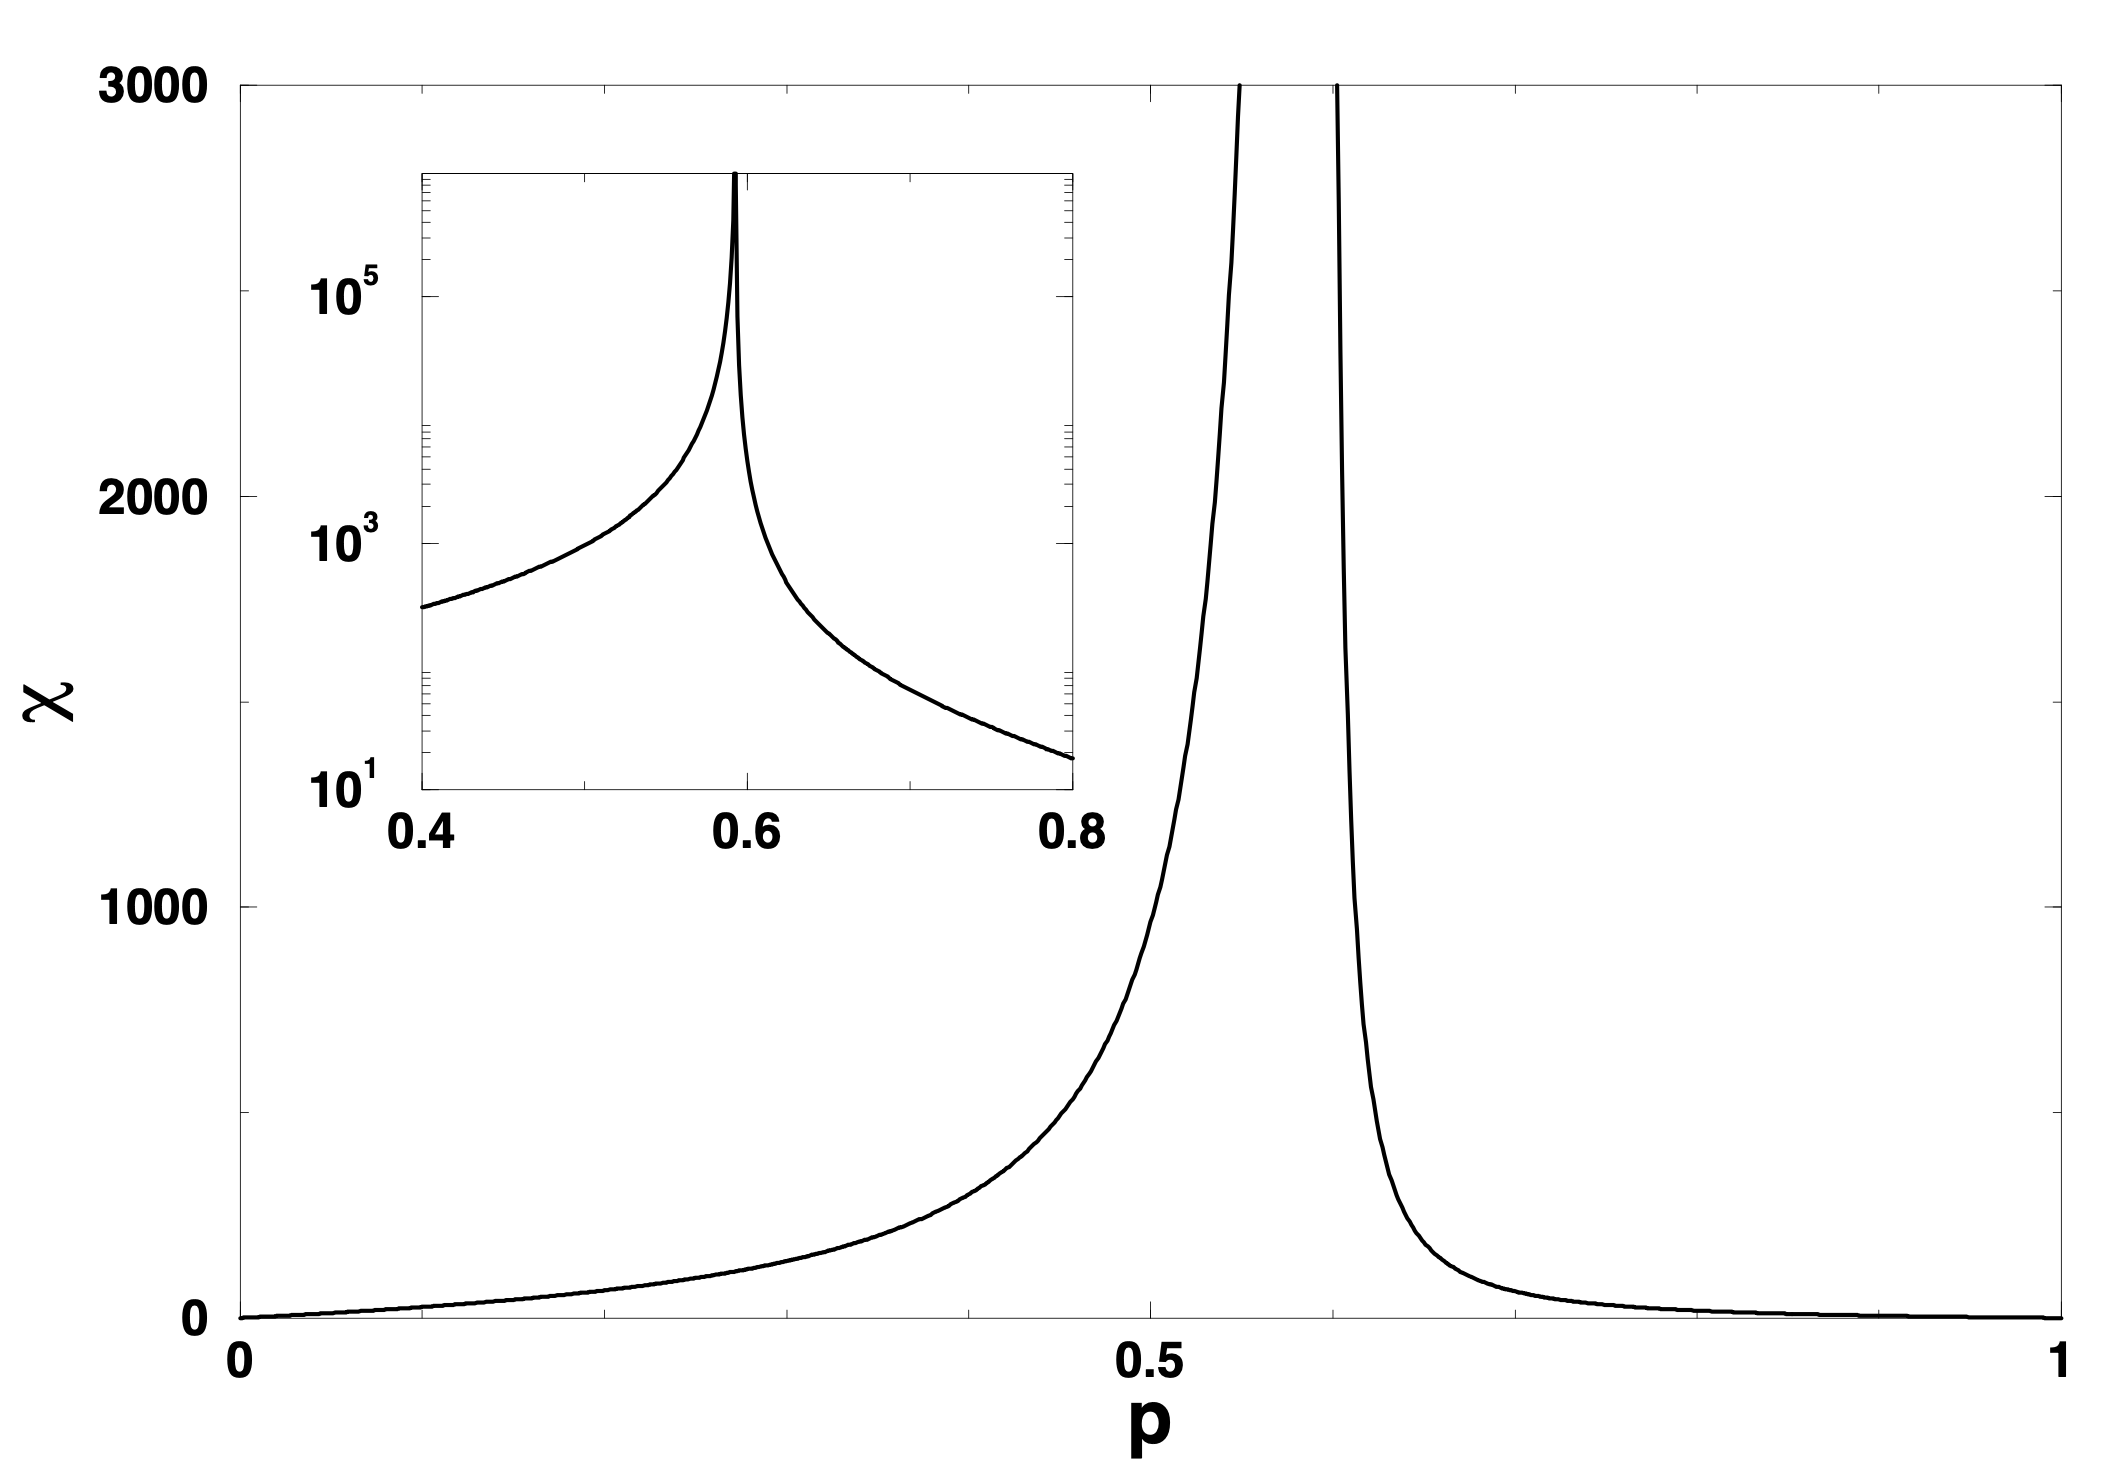
\includegraphics[width=\linewidth]{Images/mean_cluster_size_1.png}
  \caption{Percolation probability curve for various lattice sizes}
  \label{fig:mean_cluster_size_1}
\end{figure}


Again, analogously to the percolating cluster strength $P(p)$, $\gamma$ is a universal critical exponent, in the sense that it's independent of the local geometry, and depends only on the dimension of the lattice. In two dimensions, $\gamma = \frac{43}{18}$. One important difference between $\chi(p)$ and $P(p)$, however, is that $\chi(p)$ scales as $|p - p_c|^\gamma$ for both $p < p_c$ and $p > p_c$. The constants of proportionality are different in either side.


\section{Correlation function and correlation length} 

The correlation function $g(\vec{r})$ encodes how likely it is that two clusters separated by a displacement vector $\vec{r}$ are part of the same (finite) cluster. In 2D,  based on rotational symmetry and in order to simplify the analysis, one often ignores the vector character of  $\vec{r}$ and studies only $g(r)$, where $r = |\vec{r}|$.


For large values of $r$ and $p \neq p_c$, the correlation function decays exponentially: 

$$ 
    g(r) \propto e^{-\frac{r}{\xi(r)}} \textrm{,} \hspace{0.35cm}  \textrm{for} \hspace{0.15cm} p \neq p_c, \hspace{0.15cm} r \gg 1 
$$ 

$\xi(r)$ is the so called correlation length. One interpretation is that it measures the size of correlations in the lattice, that is, the typical diameter of an island. With this interpretation, one does not need to consider distances larger than $\xi$: a finite piece of the lattice, larger than $\xi$, presents the same behavior as an infinite lattice. 

This exponential form is only the leading factor in $g(r)$. At $p = p_c$, long range correlations appear, $\xi(p)$ diverges, and a power law leading factor appears:

$$ 
    g(r) \propto x^{-\eta} \textrm{,} \hspace{0.35cm}  \textrm{for} \hspace{0.15cm} p = p_c, \hspace{0.15cm} r \gg 1 
$$ 


Once more, the critical exponent $\eta$ is universal. In 2D, $\eta = \frac{5}{24}$. 

When $p \neq p_c$, the correlation length defines a characteristic length scale. This is not the case when $p = p_c$: there's no characteristic length scale. The lattice is self similar and any finite piece is not enough to describe the behaviour of the system.

Near the threshold $p_c$, the correlation length, again, behaves like 

$$ 
    \xi(p) \propto  |p - p_c|^{-\nu} \textrm{,} \hspace{0.35cm}  \textrm{for} \hspace{0.15cm} |p - p_c| \ll 1 
$$ 

with $\nu$ the corresponding critical exponent, also universal. In 2D, $\nu = \frac{4}{3}$.

It is interesting to notice here the importance of considering only finite clusters: the correlation length remains finite both below and above the threshold $p_c$. As we increase $p$ past $p_c$, finite clusters begin forming connections to the infinite cluster, and so the probability that two nodes belong to the same finite cluster (which is what $g(r)$ measures) decreases, and so does the correlation length.  

\section{Cluster size distribution} 

Perhaps the most important quantity we'll look at is the cluster size distribution, $n(s, p)$. This function describes the s-cluster density at occupation probability $p$, that is, the number of clusters with size $s$ and probability $p$ divided by the size of the lattice (in the case of infinite lattices, this quantity can be thought of either as an average over many large finite pieces of the infinite lattice, or as a limit as $L \rightarrow \infty$. At $p_c$, the the cluster size follow a power law distribution:

$$
    n(s, p_c) \propto s^{-\tau}
$$

where $\tau$ is another universal exponent (in two dimensions, $\tau = \frac{187}{91}$). Once more, the system lacks a characteristic length scale. 
Near $p_c$ and for large s, $n(s, p)$ is a generalized homogeneous function of $p - p_c$ and $\frac{1}{s}$. 

A function of two variables $F(x, y)$ is said to be generalized homogeneous function iff 

$$ 
F(c^\alpha x, c^\beta y) = c F(x, y) \hspace{0.35cm} \forall (c, \alpha, \beta)
$$

In the case of $n(s, p)$, we have 

$$
    n\bigg(\frac{c^\alpha}{s}, (p-p_c)c^\beta\bigg) = c n\bigg(\frac{1}{s}, p-p_c\bigg)
$$


By choosing $c = s^\frac{1}{\alpha}$, one obtains 


$$ 
n(1, (p-p_c) c^{\beta / \alpha}) =  n((p-p_c) c^{\beta / \alpha}) = s^\frac{1}{\alpha}n\bigg(\frac{1}{s}, p-p_c\bigg)
$$ 

which allows us to conclude that 

$$ 
n(1/s, p - p_c) = s^{-1/\alpha} n\big((p - p_c) c^{\beta / \alpha}\big)
$$ 

What this means is that by measuring $n(s, p)$ in units of $n(s, p_c)$, that is, by taking $\frac{n(s, p)}{n(s, p_c)}$ one does not need to consider it as a function of two variables $p$ and $s$: it reduces to a function which depends only on the combination $(p - p_c)s^\sigma$ for some sigma. In 2D, $\sigma = \frac{36}{91}$, which is also a critical exponent. 


One of the reasons why $n(s, p)$ is one of the most interesting quantities to look at is that the order parameter (the percolating cluster strength), the mean finite cluster size, the correlation length and other quantities can all be derived from it. For this reason, $n(s, p)$ is called a generating function.

The percolating cluster strength $P(p)$, for example, can be obtained from 

\begin{equation}
P(p) = p - \sum_s s\, n(s, p)
\end{equation}

$n(s, p)$ describes the s-cluster count divided by the size of the lattice. So $s\, n(s, p)$ can be viewed as the total area proportion covered by all clusters of size $s$. In other other, it represents the probability that by picking a node at random, it will be part of an $s$ cluster. By summing over all (finite) values of $s$, we get the probability that a randomly picked node belongs to a finite cluster. Since $p$ can be viewed as representing the probability of belonging to any cluster (since any
alive cell will, necessarily, belong to a cluster, and any node belonging to a cluster must be alive, these are equivalent descriptions), the difference between $p$ and $\sum_s s\, n(s, p)$ gives us the probability of belonging to an infinite cluster, which is how $P(p)$ is defined.


The mean cluster size $\chi(p)$ is related to $n(s, n)$ through 

\begin{equation}
    \chi(p) = \sum_s s^2\, n(s, p)
\end{equation}

As noted before, $s\, n(s, p)$ represents the probability that a randomly picked node belongs to a (finite) s-cluster. Therefore, $\sum_s s^2\, n(s, p)$ represents the expected value of $s$.

